\documentclass[a6paper, 11pt, parskip=half, DIV=15]{scrartcl}

\usepackage[dvipsnames]{xcolor}
\usepackage{tikz}

\usepackage{ragged2e}
% Minimize unwanted hyphenation
\tolerance=1
\emergencystretch=\maxdimen
\hyphenpenalty=1
\hbadness=10000

\usepackage{fontspec}
\setmainfont{URWClassico}
%\setmainfont{Qwigley}

\setkomafont{section}{\setmainfont{Cinzel-Bold}\LARGE}
\setkomafont{subsection}{\setmainfont{Cinzel-Bold}\Large}
\setkomafont{subsubsection}{\setmainfont{Cinzel-Bold}\large}

% Adjust spacing before and after section headings
\RedeclareSectionCommand[
  runin=false,
  beforeskip=1.0\baselineskip,
  afterskip=-0.0\baselineskip
]{section}

% Adjust spacing before and after subsection headings
\RedeclareSectionCommand[
  runin=false,
  beforeskip=1.0\baselineskip,
  afterskip=-0.0\baselineskip
]{subsection}

% Adjust spacing before and after subsubsection headings
\RedeclareSectionCommand[
  runin=false,
  beforeskip=1.0\baselineskip,
  afterskip=-0.0\baselineskip
]{subsubsection}


\usepackage{enumitem}
\setlist[description]{labelindent=0pt, labelsep=\widthof{ }, leftmargin=\widthof{\textbf{License: }}, font=\setmainfont{URWClassico}\bfseries}

\usepackage[hang,flushmargin]{footmisc}
\newcommand\blfootnote[1]{%
  \begingroup
  \renewcommand\thefootnote{}\footnote{#1}%
  \addtocounter{footnote}{-1}%
  \endgroup
}

\renewcommand{\thefootnote}{\fnsymbol{footnote}}
\renewcommand{\footnoterule}{%
  \kern -3pt
  \hrule width \textwidth height 0.5pt
  \kern 2pt
}

\usepackage[hidelinks]{hyperref}
\usepackage[type={CC}, version={4.0}, modifier={by-sa}]{doclicense} % Add text and icons for creative commons license
%\usepackage{array}

\raggedright
\pagestyle{empty}
\begin{document}

\begin{titlepage}
\enlargethispage{3.0\baselineskip}
%\setmainfont[Scale=2.1]{DarkCrystal-Outline}
\setmainfont[Scale=1.65]{DarkCrystal-Regular}
\Huge
\begin{center}
\vspace*{-0.5\baselineskip}
Parliament

of Dragons
\vfill
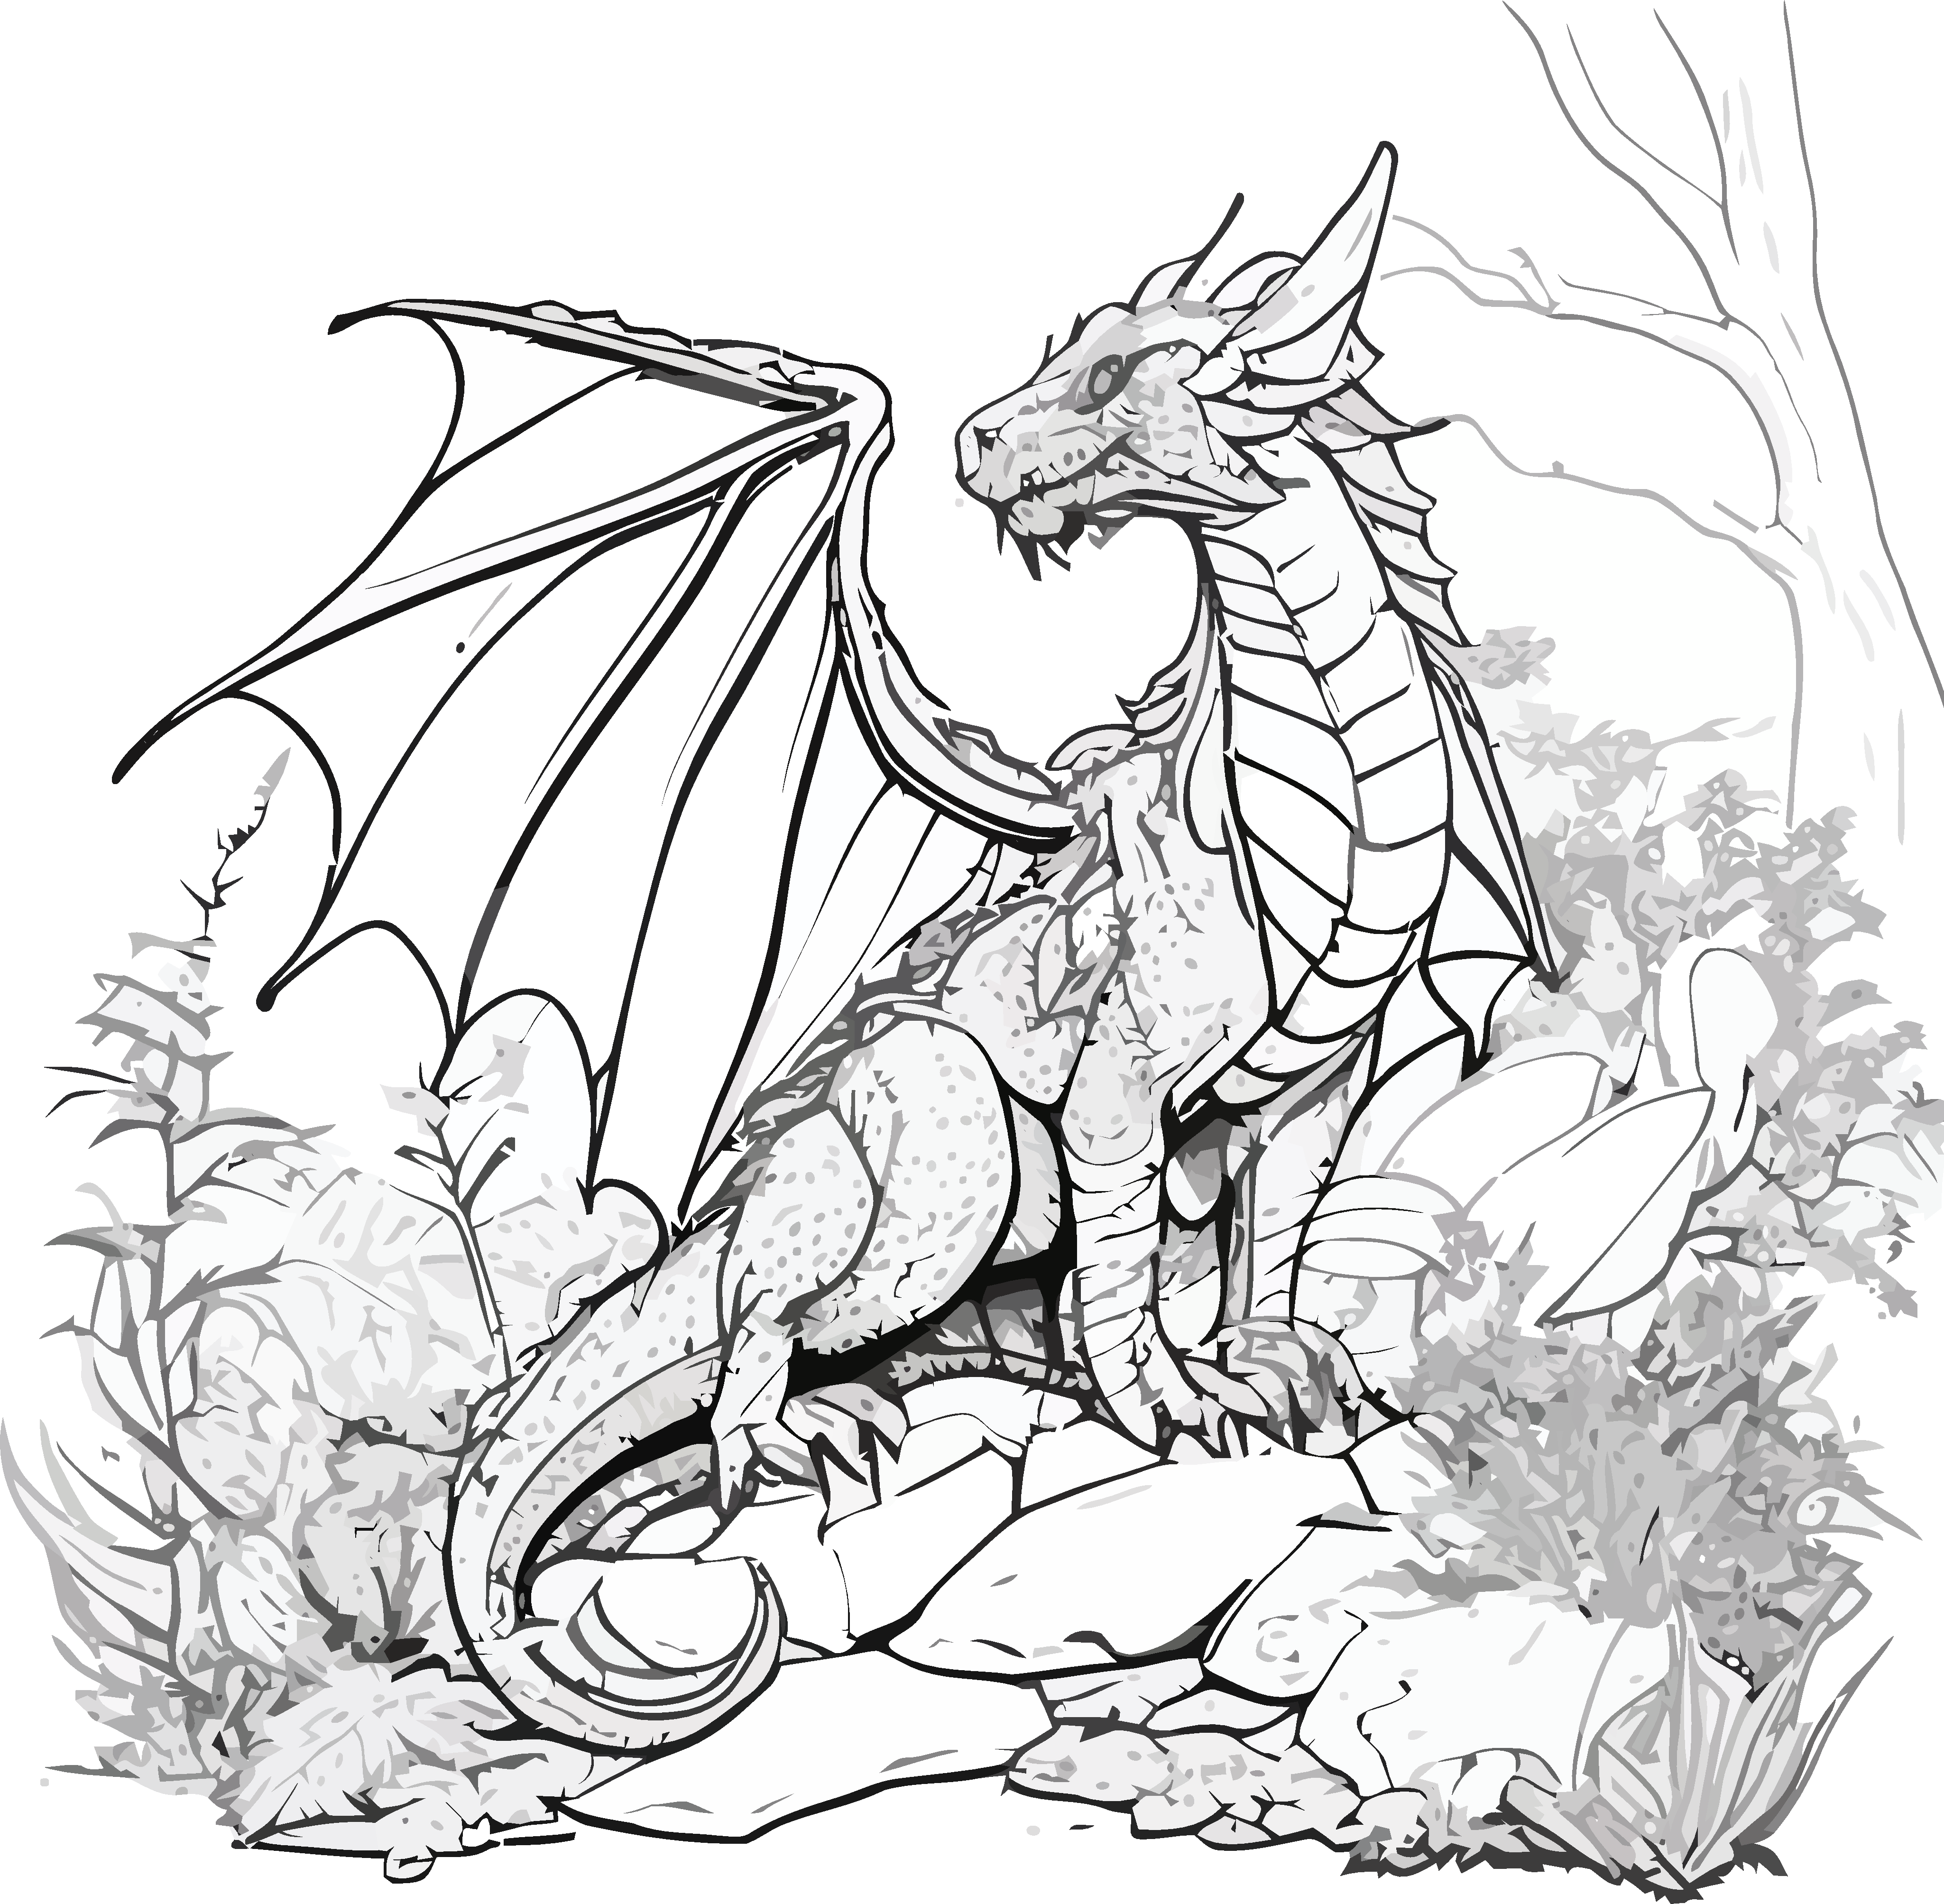
\includegraphics[scale=0.075]{Images/dragon_on_rocks.png}
\vfill
\huge
%\setmainfont{Cochin}
\setmainfont{Tex Gyre Chorus}
A Socratic Worldbuilding Game\\
\setmainfont{Tex Gyre Chorus}
by Michael Purcell
\end{center}
\end{titlepage}
\thispagestyle{empty}
\enlargethispage{1.75\baselineskip}
\setmainfont[Scale=2.0]{Tex Gyre Chorus}
\Huge
\begin{center}
Dragonhome
\smallskip
\vfill
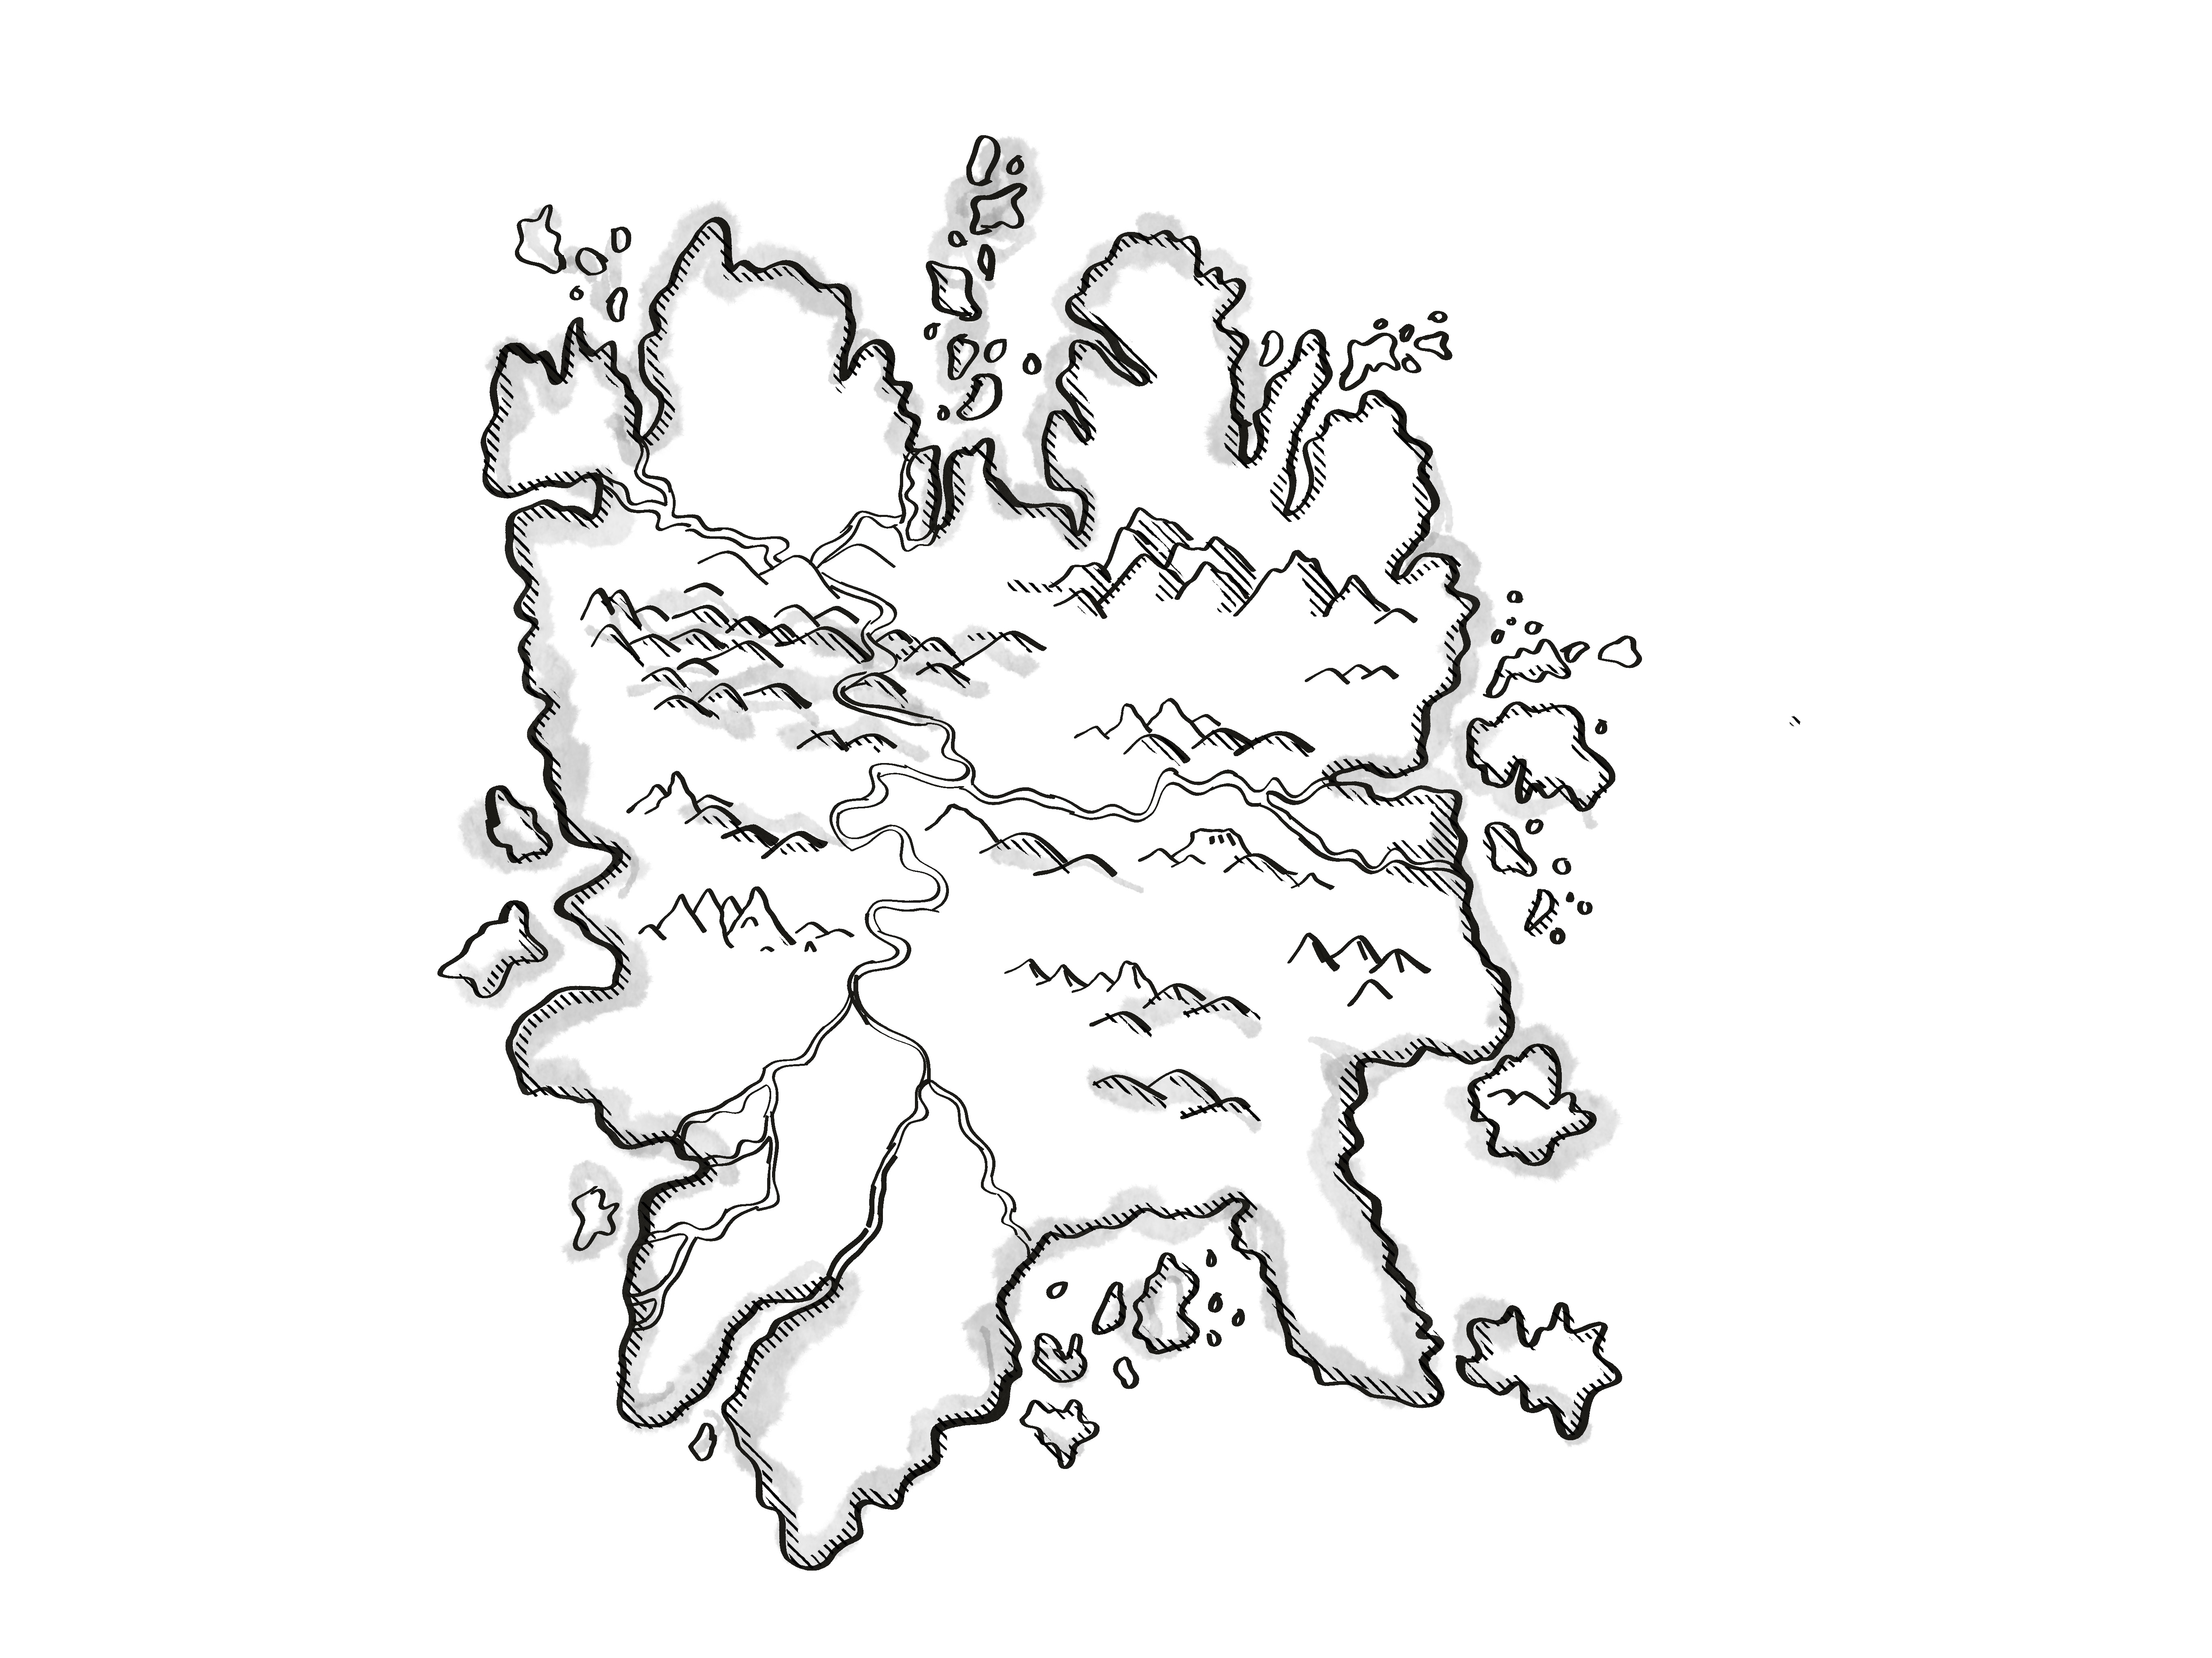
\includegraphics[scale=0.33]{Images/island_map.png}
\end{center}
\setmainfont[Scale=1.0]{URW Classico}
\normalsize

\newpage
\enlargethispage{3.5\baselineskip}

\section*{Overview}
This is a worldbuilding game. It is intended for groups of three to six players and can be played in about one hour.

You will assume the roles of dragons who have long been the undisputed rulers of Dragonhome, the island continent on which you reside. Recently, however, a fleet of ships carrying settlers from afar arrived and they have begun establishing a new colony. You have gathered in a rare Parliament of Dragons to discuss the situation and decide how you want to respond.

During the game, you will address a series of questions about the colonists and how their arrival will affect life on Dragonhome. You will invent the answers to these questions as you play. By doing so, you will describe the world in which your characters live, who the colonists are, and why they have encroached upon your domain.


\newpage
\enlargethispage{1.75\baselineskip}
\section*{Characters}
You will portray a dragon who is one of the rulers of Dragonhome. To create your character,
\begin{enumerate}[nosep]
	\item Describe the lands and creatures on Dragonhome that you claim as your own.
	\item Describe your background, mannerisms, and physical appearance.
	\item Describe two types\footnote[1]{This is intentionally vague. If in doubt, pick any two of the\\standard interrogatives (see {\setmainfont{Cinzel-Bold}\scriptsize Factual Questions} for details).}of questions about the colonists that you can answer.
	\item Describe one problem that the colonists have caused and that you would like to solve.
\end{enumerate}
Introduce yourself to the other characters before the meeting begins.

\section*{Miniatures}
Use miniatures of some kind to represent your dragon characters. You should collectively decide whose miniature is most impressive. That player's character will be the alpha dragon among the rulers of Dragonhome. 

\newpage
\enlargethispage{1.75\baselineskip}
\subsection*{Decorum}
The alpha dragon has the responsibility to ensure, however they deem appropriate, that everyone has a fair chance to contribute and that the discussion stays focused on the topic at hand. %In addition to their administrative duties, the facilitator may (and should) contribute to the discussion via their character as usual. 

\section*{Gameplay}
The game takes place over a series of five rounds. 
During each of the first four rounds, you will discuss one of the topics of interest.
During the last round, you will discuss how to respond to the issues raised in previous rounds. 

\subsection*{Topics}
There are four topics of interest:
\begin{enumerate}[nosep]
	\item Stealing the colonists' treasure.
	\item Instilling fear into the hearts of the colonists.
	\item Eating the colonists and/or their livestock.
	\item Demonstrating the power and majesty of the dragons of Dragonhome to the colonists.
\end{enumerate}
In each of the first four rounds, you will discuss one of these topics.

\newpage
\enlargethispage{1.75\baselineskip}

\subsection*{Questions}
During the game, you will ask and answer questions both about the colonists and about the game's setting.
You will invent the answers to these questions as they arise to describe the world that your characters inhabit.

\subsubsection*{Factual Questions}
Factual questions are questions about the nature of some part of the game's setting.
These questions are usually stated using a standard interrogatives: who, what, where, when, why, or how.

Whoever is best suited to answer each factual question should do so.
Your answers should be consistent with any details about the setting that have been previously established.
Beyond that, however, you are free to invent any details you like as a part of your answers.

\newpage
\enlargethispage{1.75\baselineskip}

\subsubsection*{Socratic Questions}
Socratic questions are questions that encourage critical thinking.
These questions frequently arise as follow-up questions after a player establishes a new detail about the game's setting.

Socratic questions are often intended to do one or more of the following:
\begin{itemize}[nosep]
	\item Clarify concepts
	\item Challenge assumptions
	\item Probe evidence
	\item Discover alternative viewpoints
	\item Explore implications
\end{itemize}

After someone answers a factual question, you should use Socratic questions to help them flesh out their answer and explain how any new details they introduced interact with other details that had been previously established.

\newpage
\enlargethispage{1.75\baselineskip}

\subsection*{Taking Action}
During the last round, your job is to decide what you are going to do next.
You should describe what you think needs to be done, what you can do yourselves, and what you need help with.
\blfootnote{\textbf{Contact}: \href{mailto:pod.ttrpg@gmail.com}{pod.ttrpg@gmail.com}}
\blfootnote{\textbf{License}: \raggedright\doclicenseLongText}

As in the previous rounds, you should use Socratic questions to help each other understand what you are proposing and why your proposal describes a reasonable course of action.

\vfill

\begin{center}
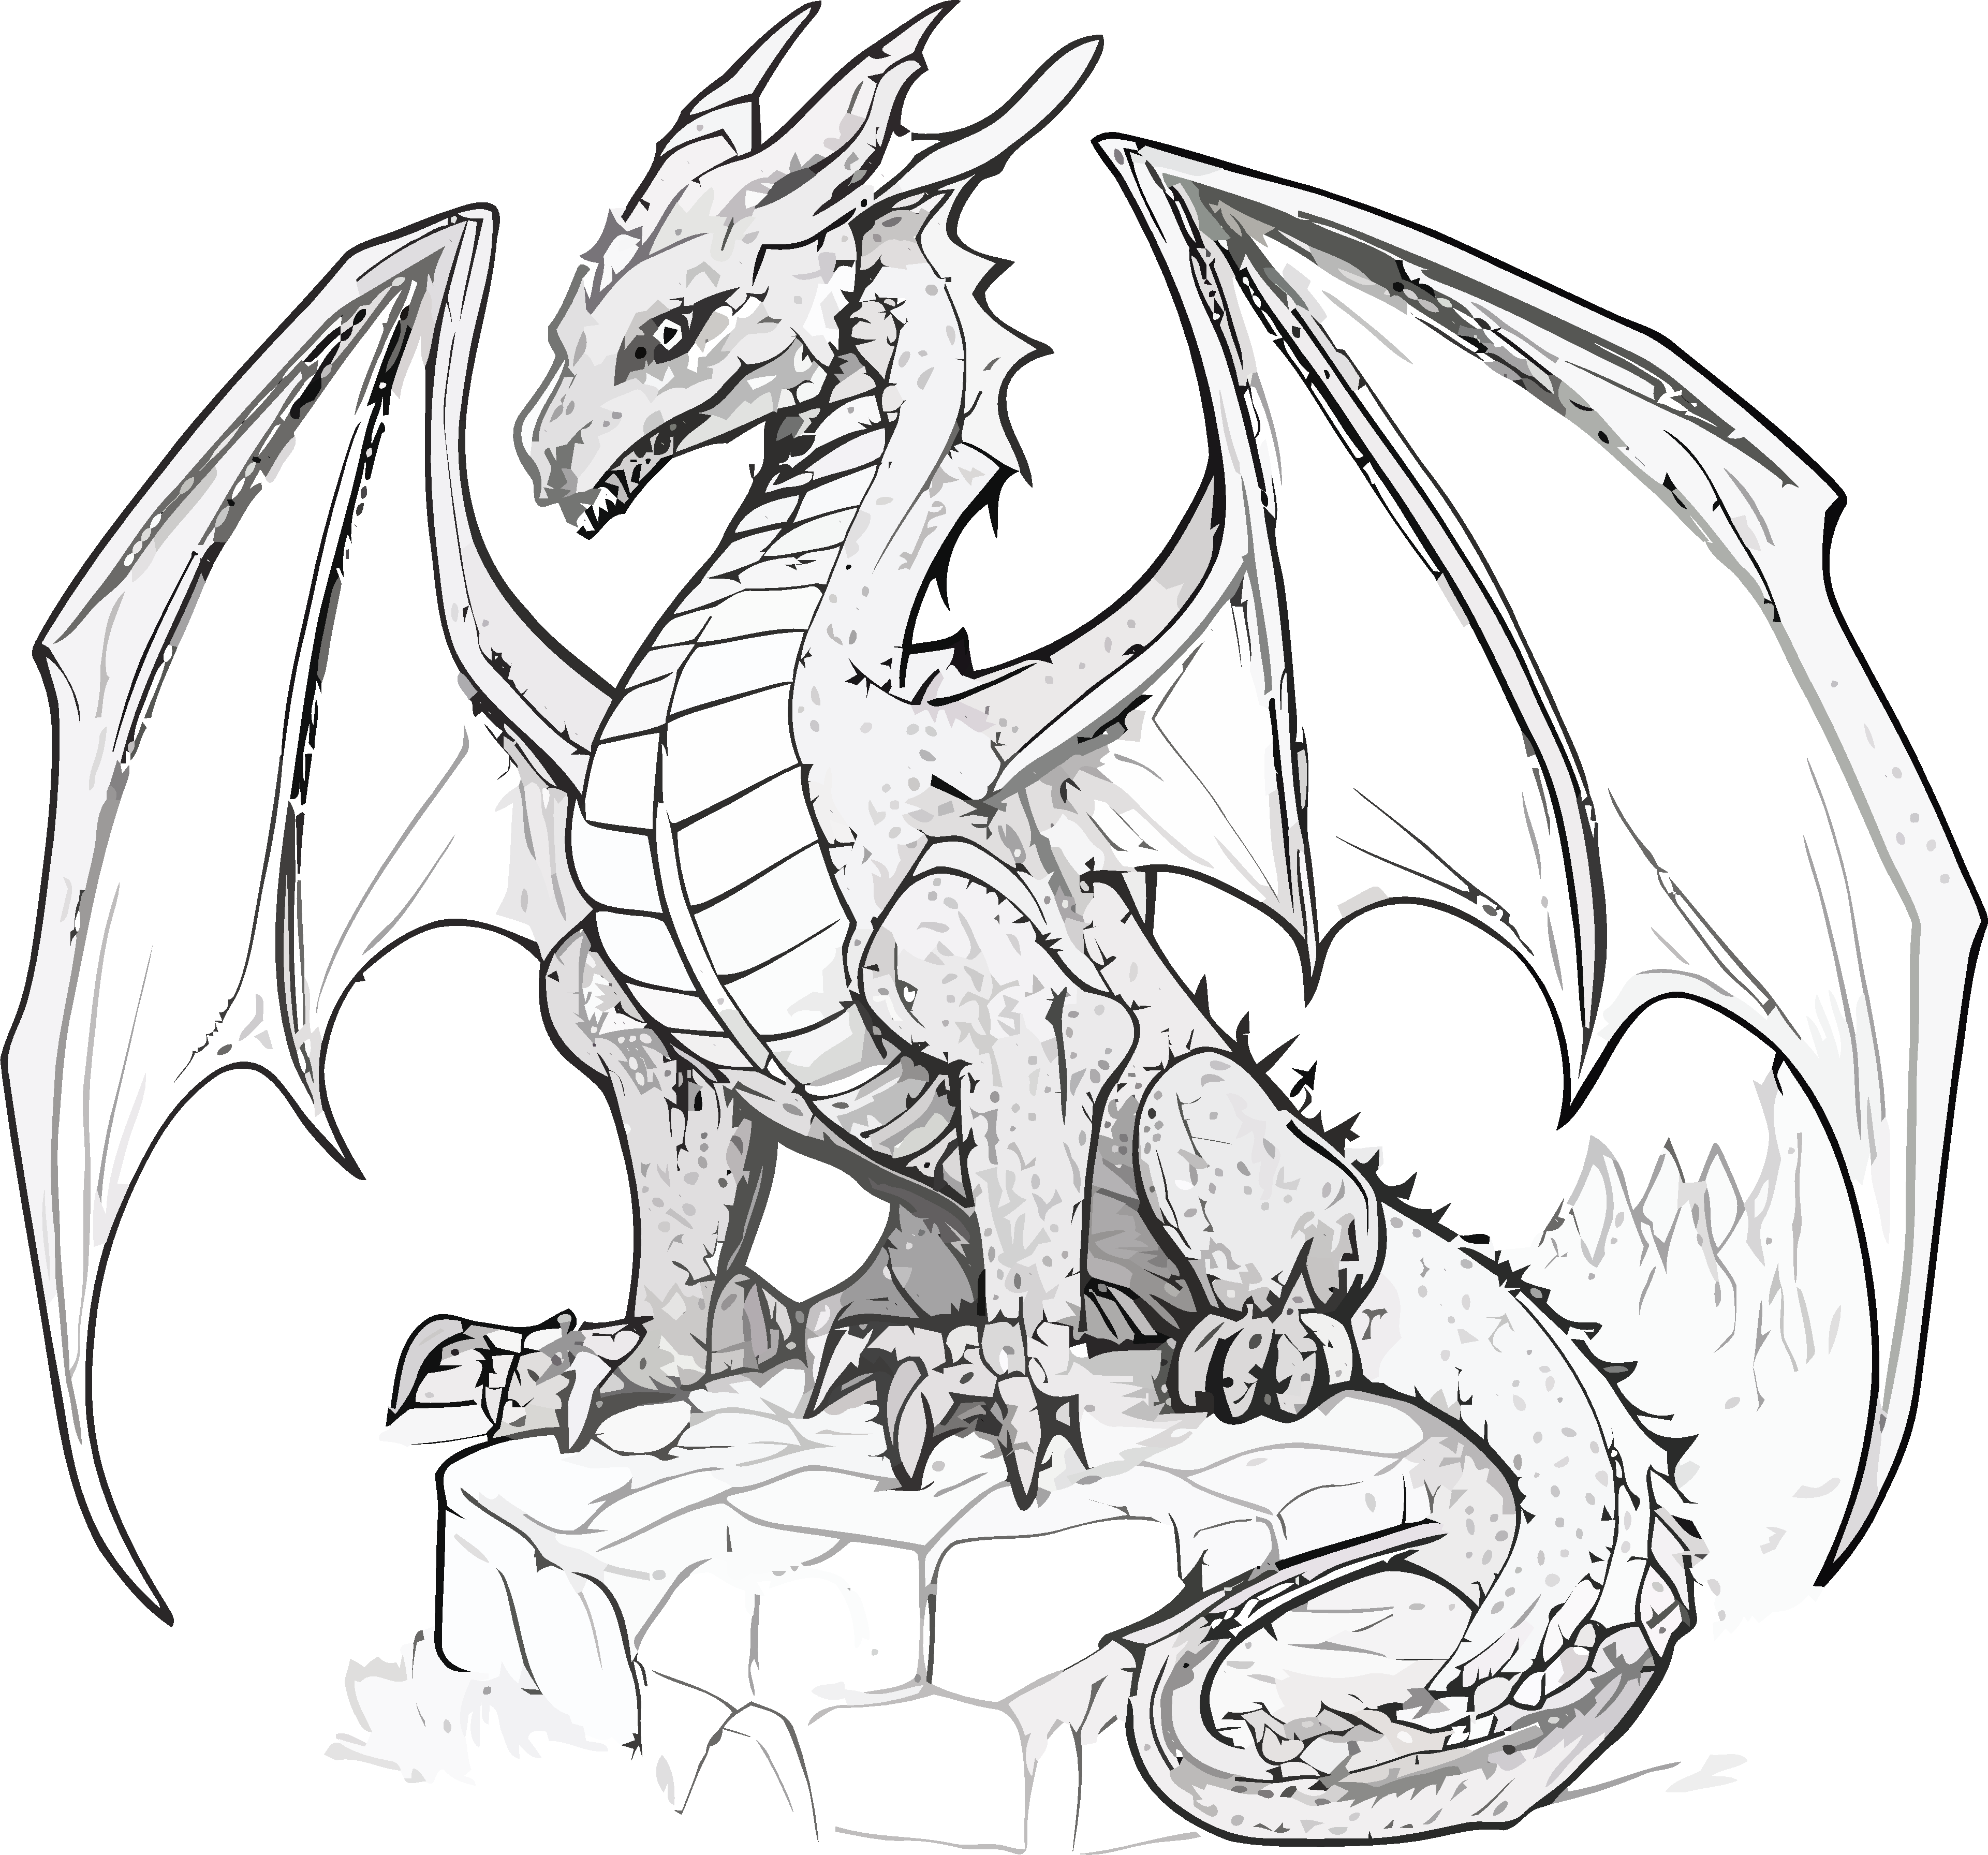
\includegraphics[scale=0.0625]{Images/dragon_on_rocks2.png}
\end{center}

\vfill

\end{document}